\section{3-Majority}
\label{3Majority}
In this transition rule, as we have already written, the selected agent u observes the opinions of three other agents selected uniformly at random. It then adopts the majority among the sample, breaking ties randomly.
Also for this transition rule, we have done the same plots that we have presented for the 2-Choice transition rule. So we pass immediately to the analysis of them.
But before showing the plots we can say that we would expect that the algorithm is faster compared to 2-Choices. In fact in this way we break ties randomly and especially at the beginning the algorithm should go faster. This anticipation stems from the random breaking of ties, especially in the initial stages of the algorithm.

\begin{figure}[H]
     \centering
     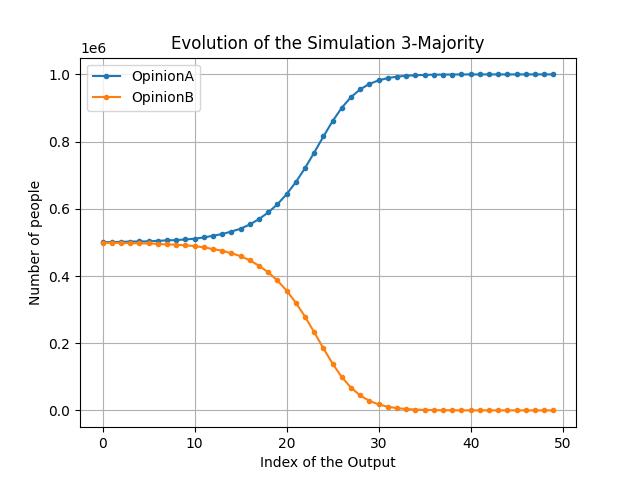
\includegraphics[width=0.78\textwidth,height=0.32\textheight]{img/svg/3_Majority/1mln/withoutTime.png}
     \caption{Simulation done with 1mln agents, output each 500 000 iterations}
\end{figure}
\begin{figure}[H]
     \centering
     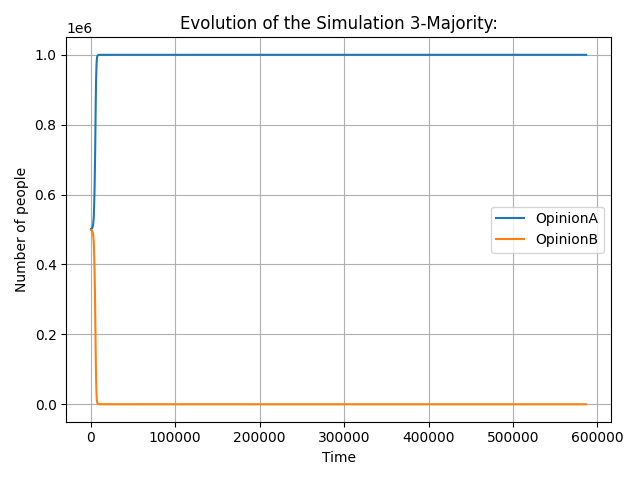
\includegraphics[width=0.75\textwidth,height=0.32\textheight]{img/svg/3_Majority/1mln/withTime.png}
     \caption{Simulation done with 1mln of agents, Time calculated in ms}
\end{figure}

The reason between the difference of these two plots is the same as we have already presented in the Chapter of 2-Choices.

\begin{figure}[H]
     \centering
     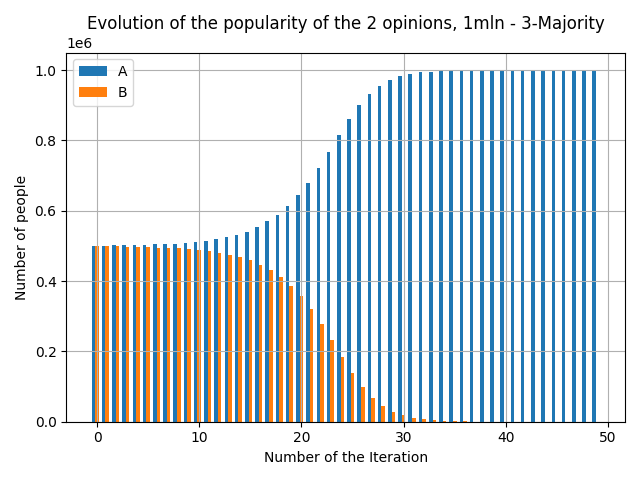
\includegraphics[width=0.80\textwidth,height=0.37\textheight]{img/svg/3_Majority/1mln/barChart.png}
     \caption{Simulation done with 1mln of agents}
\end{figure}

On the other hand, in this plot we can see something really interesting. As we expected, especially in the first steps of the algorithm, it goes faster than the 2-Choices’ simulation, for the reasons that we have already talked about.\\

The plots below show the behavior of the algorithm with 10mln and 100mln of agents. As we can see the evolution of the line is approximately the same as with 1mln agents, for this reason there isn’t much to say about them.

\begin{figure}[!ht]
     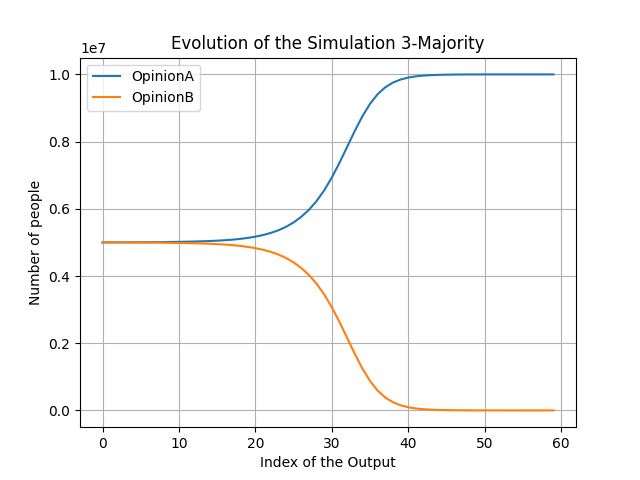
\includegraphics[width=0.40\textwidth,height=0.17\textheight]{img/svg/3_Majority/10mln/withoutTime.png}
     \centering
     \includegraphics[width=0.40\textwidth,height=0.17\textheight]{img/svg/3_Majority/10mln/withTime.png}
     \caption{Simulation done with 10mln agents, Time in ms}
\end{figure}
\begin{figure}[!ht]
     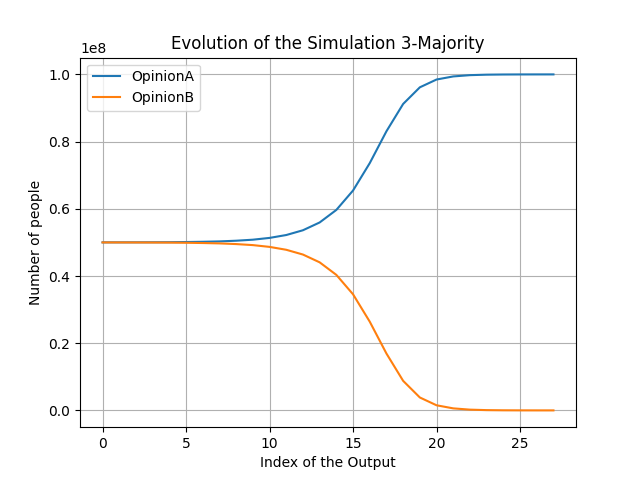
\includegraphics[width=0.40\textwidth,height=0.16\textheight]{img/svg/3_Majority/100mln/withoutTime.png}
     \centering
     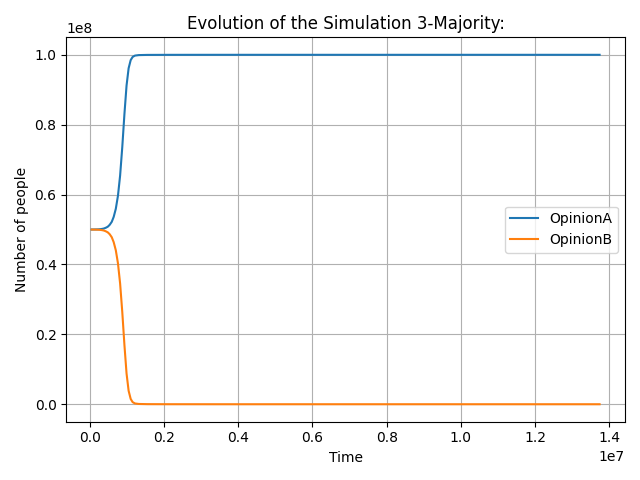
\includegraphics[width=0.40\textwidth,height=0.16\textheight]{img/svg/3_Majority/100mln/withTime.png}
     \caption{Simulation done with 100mln agents, Time in ms}
\end{figure}

At the end, as we have already mentioned in the 2-Choices chapter, the time and the number of agents are directly proportional, but not of the same factor! In fact between 10mln and 100mln the factor between the two times needed by the simulation is approximately a little more than 1/3 , that is way less than 1/10, which is the factor between 10 and 100 million. This thing can be seen in the following bar chart.


\begin{figure}[H]
     \centering
     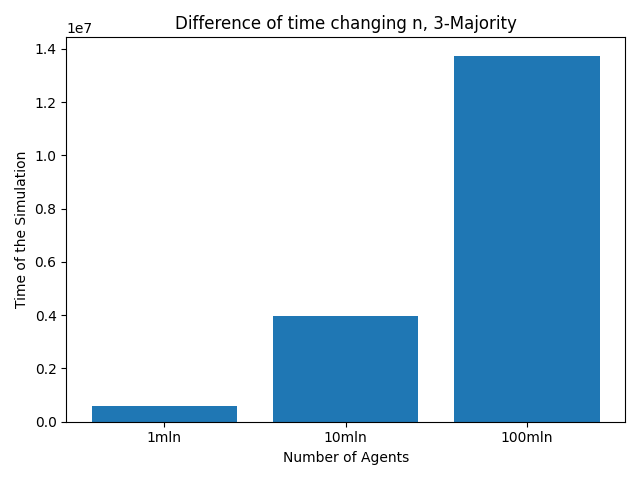
\includegraphics[width=0.80\textwidth,height=0.37\textheight]{img/svg/3_Majority/TimeDifferenceN.png}
\end{figure}
\newpage

\subsection[0.5-0.75 3Majority]{Comparison between 0.5 and 0.75, 3-Majority simulation}
Similarly, the instances decreased for the 3 majority model as well. The time decreased to 1 million from 4 million, when the ratio is set as 0.75. And the new number of iterations was 115,000,000, while the old one was around 300,000,000.
\begin{figure}[H]
     \centering
     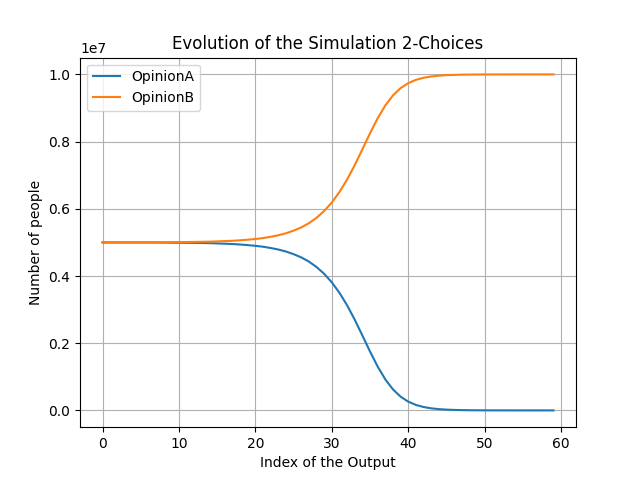
\includegraphics[width=0.60\textwidth,height=0.23\textheight]{img/svg/0.75/3-Majority/withoutTime.png}
     \caption{Probability A 0.75, output each 5 million iteration}
\end{figure}
\begin{figure}[H]
     \centering
     \includegraphics[width=0.60\textwidth,height=0.23\textheight]{img/svg/0.75/3-Majority/withTime.png}
     \caption{Probability A 0.75, Time calculated in ms}
\end{figure}
\begin{figure}[H]
     \centering
     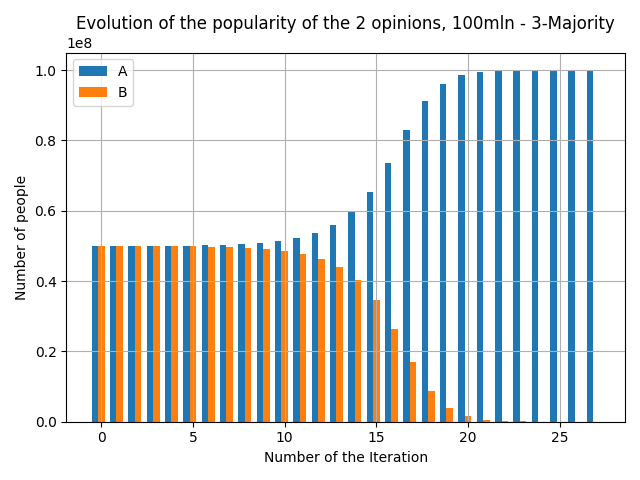
\includegraphics[width=0.60\textwidth,height=0.23\textheight]{img/svg/0.75/3-Majority/barChart.png}
     \caption{Probability A 0.75, Done with 10mln of agents}
\end{figure}